% !TEX root = ../main.tex

\chapter{Introduction}

\section{Image Segmentation}
The human brain is able to process information captured by our eyes and learn a remarkably rich representation of the world around us. However, developing an artificial system that can achieve the same performance and robustness has long challenged researchers from very diverse fields like psychology, physiology, engineering, computer science, and artificial intelligence.

\emph{Computer vision} is a multidisciplinary field of science that enables computers to gain high-level understanding from digital images, videos, and other visual inputs. 
The idea of ``understanding digital images'' usually means deriving a compressed and meaningful description of the images that can then be used for further analysis.
A typical example is the task of image classification, where an image is assigned to exactly one label from a fixed set of classes such as \{cat, dog, person\}. 
Another important example is \emph{image segmentation}, which is the process of partitioning an image into meaningful segments or sets of pixels. 

There exist two types of image segmentation: \emph{Semantic segmentation} assigns each pixel of the image to a label from a defined set of classes (e.g. person, car, tree, sky); \emph{Instance segmentation} assigns each pixel not only to a class but also to a unique instance id so that different object instances belonging to the same class are distinguished (e.g. car-1, car-2, person-1). 
In this thesis, we focus on instance segmentation. An example of an application is the segmentation of neuronal tissue images (see Fig.~ \ref{fig:neuron_segmentation_data} and \ref{fig:segmentation_cremi_GASP}). In this task, there is only one class of objects (neuron cells), and each pixel has to be assigned to its corresponding neuron cell so that all pixels belonging to the same neuron cell are grouped together. 
% Note that the number of neuron cells is not known beforehand. 

In the following sections, we will introduce the methods and graph partitioning algorithms that are studied in this thesis, and show how they can be used to solve instance segmentation tasks such as neuron segmentation.


\newpage
\section{Deep Learning and Graph-Based Instance Segmentation}
% \TODO{Add more citations?}
In the last decade, computer vision experienced incredible progress. This was due in big part to deep learning, which is now omnipresent in the field of image analysis. As a machine learning tool, fully-connected neural networks (also known as multilayer perceptrons) encode the input through a number of non-linear fully-connected layers, where each neuron in one layer is connected to all neurons in the next layer. The neural network model's architecture is defined by the arrangement of these layers. Convolutional neural networks (CNNs) represent one of the most relevant classes of neural network architectures used in computer vision and digital image analysis. A convolutional layer of a CNN convolves its input and passes the result to the next layer. Convolution kernels shift over input features and provide in this way translation equivariant responses. As compared to fully-connected neurons, a convolutional neuron processes data only for its receptive field, remarkably reducing the number of parameters in the network and making it less prone to overfitting data.
Thanks to these properties, CNNs recently demonstrated outstanding performances at image-level understanding and recognition capabilities.

A specific type of CNN, called fully convolutional network (FCN) \cite{long2015fully}, proved to be particularly good at solving image segmentation tasks. An FCN does not include any fully-connected layer and transforms the height and width of the intermediate layers back to the input image's size. 
In this way, when applied to a semantic segmentation task, the pixel-wise class predictions of an FCN have a one-to-one correspondence with the input image in the spatial dimension.
Few years ago, an improved version of FCN was proposed, called U-Net \cite{ronneberger2015u}, which is based on an encoder-decoder structure along with long skip connections. These skip connections proved to be very successful at recovering fine-grained details in the output predictions and, recently, the U-Net model became a prevalent choice for solving image segmentation tasks in biological applications \cite{lee2017superhuman,ronneberger2015u}. In the following chapters of this thesis, we will frequently make use of the U-Net model. 

FCNs and CNNs have also been applied to instance segmentation tasks.
There are two main types of deep learning approaches to instance segmentation: \emph{proposal-based} and \emph{proposal-free} methods. 
\emph{Proposal-based} methods first perform object detection, for example by predicting anchor boxes \cite{ren2015faster}, and then assign a class and a binary segmentation mask to each detected bounding box \cite{he2017mask,porzi2019seamless}.
However, the bounding boxes predicted by these methods may overlap, which is not always desirable. 
In this thesis, instead, we study \emph{proposal-free} methods, which do not require object detection and directly group pixels into instances. 
These types of methods are preferred in imagery with object instances that cannot be approximated by bounding boxes and are much larger than the field of view of the model. 

This thesis focuses on graph-based proposal-free segmentation methods, which solve the instance segmentation task by formalizing the input image as a graph. Nodes in the graph usually represent pixels or sets of pixels (commonly named \emph{superpixels}), whereas graph edges express neighboring relationships between pixels. In these graph-based instance segmentation approaches, an FCN is trained to predict the graph's edge weights. Then, a more or less complex graph-partitioning algorithm is employed to output the final instance segmentation. 
The segmentation methods that are mostly related to this thesis predict edge weights in the form of pixel-pair affinities \cite{Gao_2019_ICCV,liu2018affinity,lee2017superhuman}, which represent how likely it is for a pair of pixels to be in the same object instance. These approaches not only predict affinities for pairs of direct-neighboring pixels in the image, but they also learn long-range pixel-pair affinities, since this proved to improve training and help the model to use large-scale features in images \cite{lee2017superhuman}.

In the following section, we will review the task of neuron segmentation in the field of connectomics, which has often been tackled by using graph-based instance segmentations methods. Then, in Section \ref{sec:graph_partitioning_intro}, we will introduce the main graph partitioning algorithms studied in this thesis.

\begin{figure}[t]
    \centering
    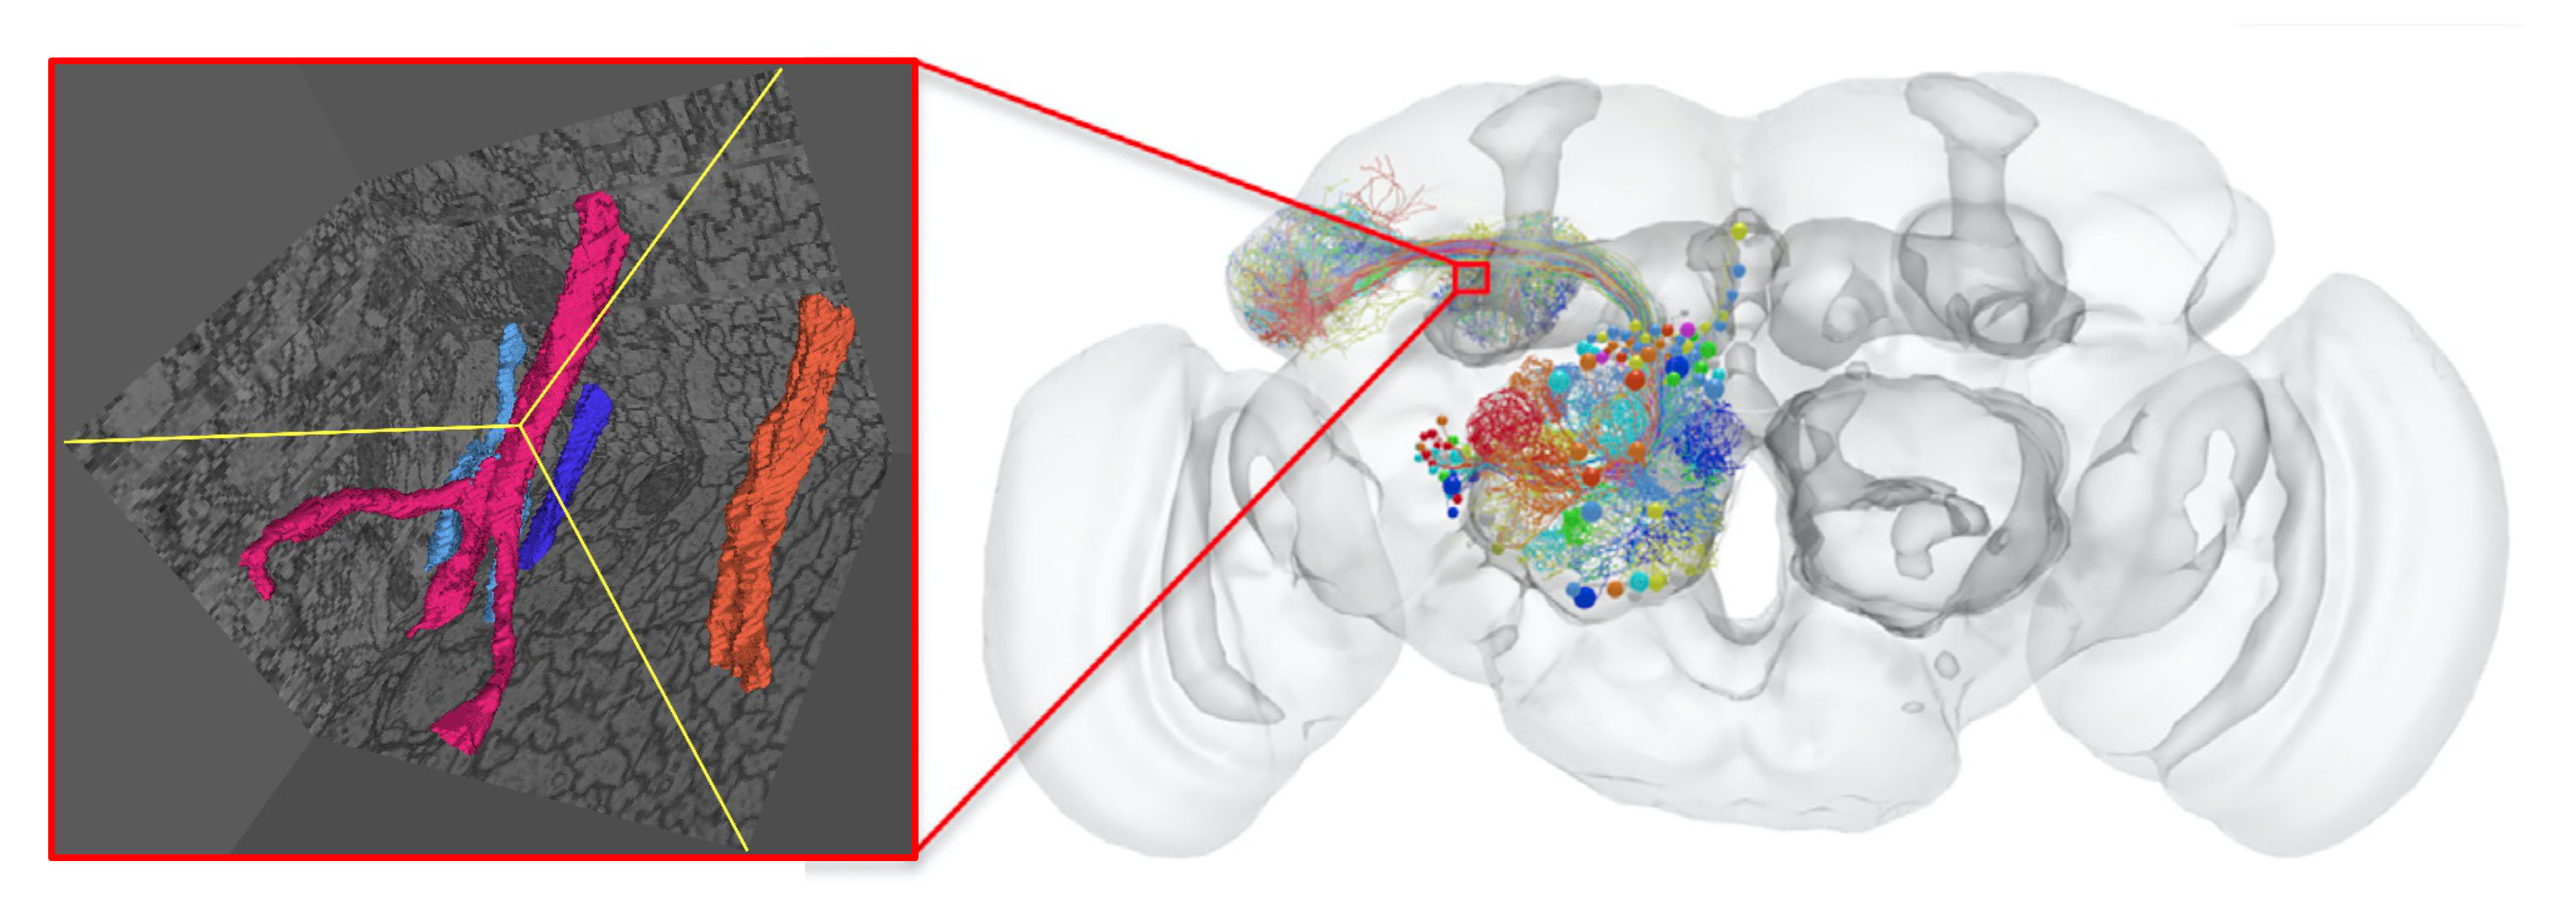
\includegraphics[width=0.95\linewidth]{figures/zoom-in-fruitfly.png}%
    \caption[Illustration of neuron reconstruction]{Reconstruction of the neural wiring diagram of the fruit-fly \emph{Drosophila melanogaster}. The neuronal processes are reconstructed from serial section transmission EM (TEM) volumes (shown on the left) of the organism's neural tissue. Four automatically reconstructed neuron instances are displayed in different colors. On the right, the ventral view of the brain is shown (image taken from \cite{zheng2018complete}).}
    \label{fig:zoom_in_fruitfly}
    % \vspace{-0.05cm}
\end{figure}


\begin{figure}[tp]
    \centering
    \includegraphics[width=0.8\linewidth]{figures/hemi-brain-data.jpg}%
    \caption[Image of neuronal tissue at different scales]{Example of electron microscopy volume image of neuronal tissue with isotropic resolution of $8 \times 8 \times 8$ nm$^3$ shown at three different scales. Data is taken from the hemibrain \cite{Xu2020.01.21.911859}: the dataset covers a large portion of the central brain of the fruit fly \emph{Drosophila melanogaster}, including the mushroom body and central complex circuits critical for associative learning and fly navigation.  Data is three dimensional. Only one 2D image from the stack is shown.}
    \label{fig:neuron_segmentation_data}
    % \vspace{-0.05cm}
\end{figure}


\begin{figure}[p]
    \centering
    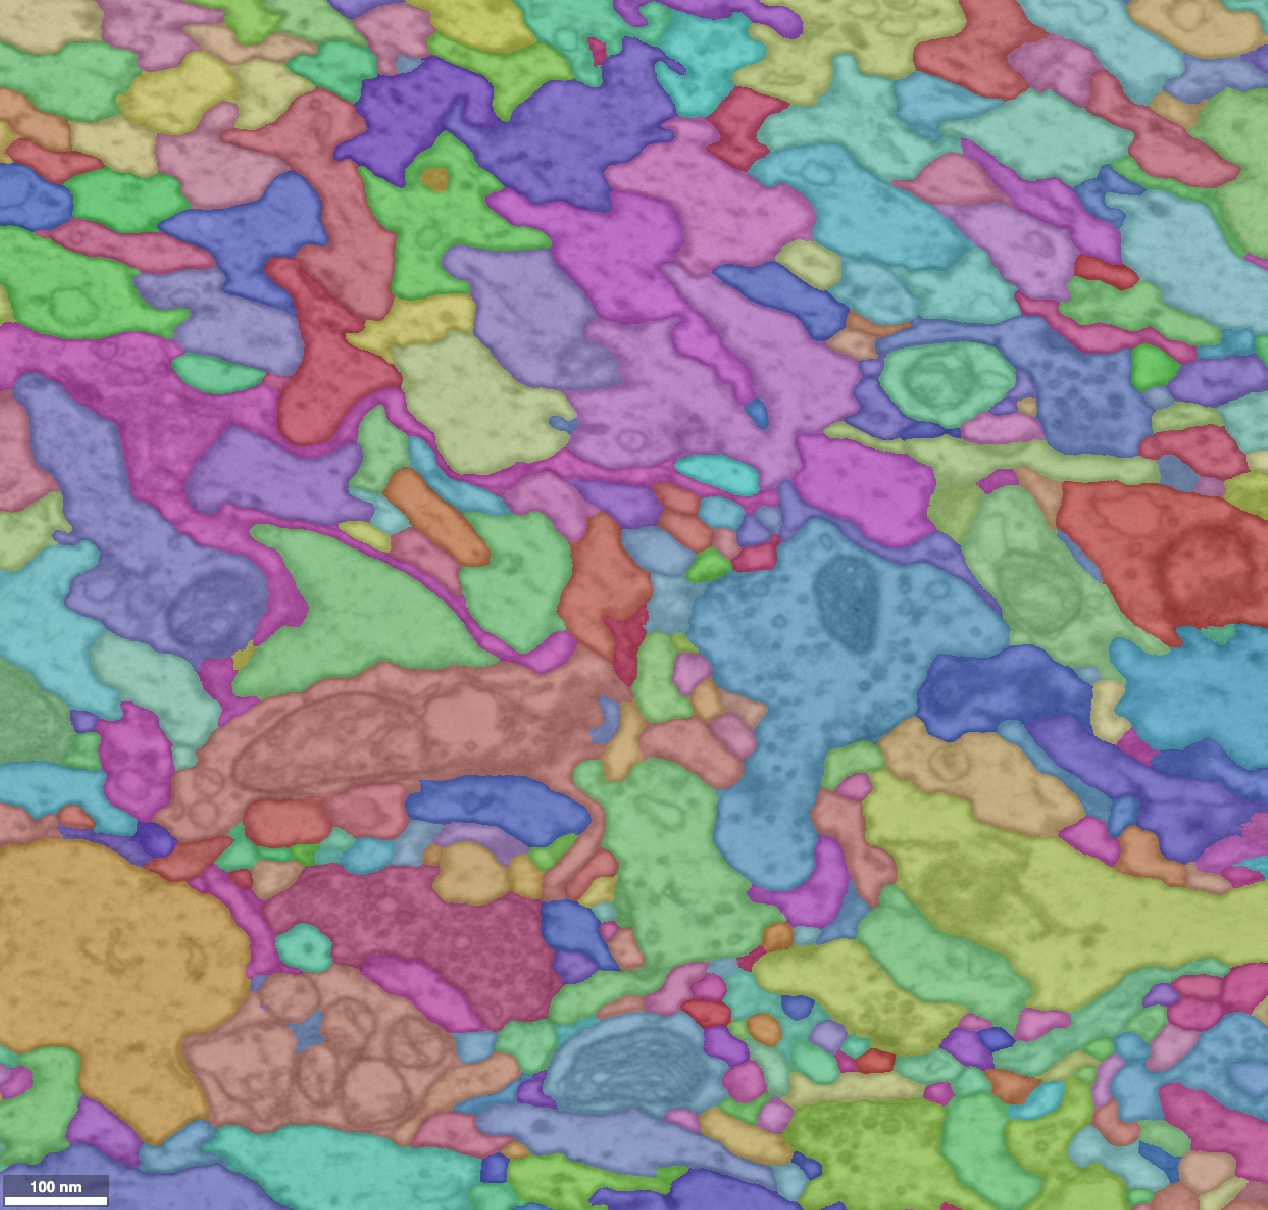
\includegraphics[width=\linewidth,trim=0 0 100 0, clip]{figures/segmentation-cremi.jpg}%
    \caption[Dense segmentation obtained with GASP and average linkage]{
Neuron segmentation data overlaid with the dense instance segmentation obtained with the method proposed in Chapter \ref{chapter:GASP} (\emph{GASP} with average linkage). Colors are randomly assigned. Note that the data is 3D, hence the same color could be assigned to parts of segments that appear disconnected in 2D. Only one 2D image from the stack is shown here. Data is taken from the test set of the CREMI neuron segmentation challenge \cite{cremi}.}
    \label{fig:segmentation_cremi_GASP}
    % \vspace{-0.05cm}
\end{figure}


 
\subsection{Neuron Segmentation in Connectomics}
Connectomics is a field of neuroscience with the goal of reconstructing the complete neural wiring diagram of an organism's central nervous system. This comprehensive map of neural connections within a brain is known as the \emph{connectome}. A fundamental step towards the reconstruction of the connectome is the segmentation of neural tissue images, which are commonly acquired using electron microscopy techniques (e.g., serial section transmission EM) yielding 3D image volumes. 

In 2017, the whole brain of an adult Drosophila melanogaster, with a volume of approximately $8\cdot 10^7 \mu m^3$ and comprising $\sim$100,000 neurons has been imaged with nanometer resolution producing a dataset of 106 TB \cite{zheng2018complete}. Similar projects are generating petabytes of data \cite{yin2020petascale}, and a mouse brain of $500$ mm$^3$, at a typical isotropic resolution of 8 nm, would require almost 1000 petabytes of data.
Despite progress in collaborative annotation \cite{kim2014space}, the sheer size of these volumes makes manual analysis infeasible. Thus, automated processing, and especially automated neuron segmentation, is needed to reconstruct the complete organism's neural wiring diagram.

The unique features of this segmentation problem, involving large volume datasets and narrow elongated neuron segments that can span big portions of an organism's brain, encouraged the development of new proposal-free instance segmentation methods.
Flood-filling networks \cite{januszewski2018high} and MaskExtend \cite{meirovitch2016multi} use a CNN to iteratively extend one neuron at a time. By using flood-filling networks, the dense connectome of half the central brain of Drosophila melanogaster, containing around 25,000 neurons, was recently reconstructed and publicly released \cite{xu2020connectome}. In order to yield sufficient accuracy for correct circuit analysis, this impressive reconstruction involved significant proof-reading efforts by expert annotators, showing that further progress is still required in automated reconstruction methods.

Another class of instance segmentation methods that proved to be particularly useful in neuron segmentation is given by graph-based segmentation approaches. 
Originally, many proposed methods predicted a boundary evidence map indicating how probable it is for every voxel to be on the boundary between two neurons. After generating superpixels and building a graph based on these boundary predictions, the final segmentation was then determined as optimal cuts on this graph \cite{andres20123d,andres2012globally,beier2017multicut,funke2018large,meirovitch2019cross,turaga2010convolutional}. Now, all of the top submissions of the CREMI \cite{cremi}, SNEMI3D \cite{SNEMI3D}, and ISBI neuron segmentation challenges employ convolutional neural networks \cite{lee2017superhuman,hirsch2020patchperpix,bailoni2019generalized}. Instead of predicting a neuron-boundary probability map, most of these methods predict affinities between voxels and directly use them to compute the edge weights of the graph \cite{lee2017superhuman,pape2017solving,hirsch2020patchperpix,pape2019leveraging,wolf2018mutex}. An alternative approach to the direct prediction of affinities was proposed by \cite{lee2019learning}, who instead learn dense voxel embeddings via deep metric learning and derive affinities in the embedded space. 

In the next section, we will review some of the graph partitioning algorithms used in these graph-based segmentation pipelines and studied in this thesis.



\section{Graph Partitioning Algorithms}\label{sec:graph_partitioning_intro}
In the previous sections, we have seen that graph-based instance segmentation methods have been successfully applied to neuron segmentation. In this section, we review the basic ideas and notation of graph-based segmentation algorithms studied in this thesis.

Usually, graph-based image segmentation methods represent the image as a graph $\mathcal{G}=(V,E)$. Each node $u\in V$ corresponds to a pixel in the image and nodes are connected by edges $(u,v)\in E$. A weight $w_e$ is associated with each edge $e \in E$ based on some property of the pixels that it connects, such as their image intensities, gradients or the output of an edge classifier (usually a neural network). Depending on the method and application, the graph might be only sparsely connected, for example as a grid graph (where every pixel is connected only its direct neighboring pixels) or a graph with limited local neighborhood connectivity.

\subsection{Agglomerative Hierarchical Clustering}
The majority of graph clustering methods work with positive edge weights representing similarities or distances between the nodes. These methods require the user to specify the desired numbers of segments or a termination criterion (as in spectral clustering or iterated normalized cuts) or even a stronger version of supervision by adding a seed for each object (e.g. in seeded watershed or random walker).  

Hierarchical clustering (HC) is another popular graph clustering method, which creates a hierarchy of clusters. Agglomerative HC is a bottom-up approach starting with each node assigned to its own cluster and incrementally merging clusters starting from those with the highest edge weight \cite{lance1967general}. As compared to other divisive partitioning algorithms (e.g. normalized graph cut), agglomerative clustering is a much more efficient method that, with a heap data-structure, has a time complexity of $\mathcal{O}(m^2 \log m)$, where $m$ is the number of edges in the graph. 

In Algorithm \ref{HC_algoritm}, we show a simplified pseudo-code describing this simple partitioning algorithm. Apart from the weighted graph, another input of the algorithm is the so-called \emph{linkage criterion}, which defines the interaction between two clusters containing multiple nodes. For example, average linkage criterion is a very common one, where the interaction between two clusters is given by the average of all the edge weights connecting them. Each time two clusters are merged by the algorithm at line 5, the interaction between the newly formed merged cluster and its neighbors has to be updated by using the given linkage criterion. 
Finally, the algorithm returns the hierarchy of clusters in the form of a \emph{dendrogram}, which is a rooted tree representing the order in which clusters were merged (see toy example in Fig.~\ref{fig:example_HC}). 

A downside of hierarchical agglomerative algorithms is that, after running the algorithm, the user has to choose a level in the cluster hierarchy in order to define the desired output clustering. 
In Chapter \ref{chapter:GASP}, we will define a framework for agglomerative algorithms that are parameter-free because they are based on graphs with both positive and negative edge weights.


\begin{figure}[t]
    \centering
    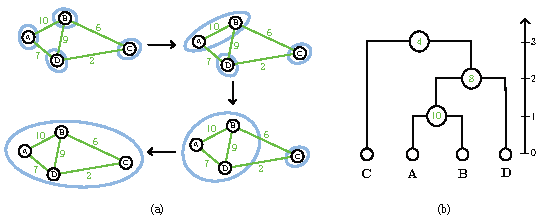
\includegraphics[width=\linewidth]{figures/example-HC.pdf}%
    \caption[Agglomerative Hierarchical Clustering demonstrated on a toy graph]{Agglomerative Hierarchical Clustering (with Average linkage criterion) on a toy graph. \textbf{(a)} On the left, the agglomeration steps of the algorithms are demonstrated on a small graph with four nodes. Edge weights are shown in green. At every step, the pair of clusters with highest interaction (according to average linkage) is merged. \textbf{(b)} On the right, the resulting dendrogram is shown, representing the merging hierarchy.}
    \label{fig:example_HC}
    % \vspace{-0.05cm}
\end{figure}
\begin{algorithm}[t]
\footnotesize
  \begin{flushleft}
  \footnotesize
  \caption{Agglomerative Hierarchical Clustering}
  % \caption{\algname{}: generalized algorithm for signed graph partitioning}
   \hspace*{\algorithmicindent} \textbf{Input:} Graph $\mathcal{G}(V,E,w)$ with affinity weights $w:E \rightarrow \mathbb{R}^+$; linkage criterion $\interact{}$ \\
  \begin{algorithmic}[1]
  \footnotesize
  % \small
      \State Initialize clustering $\{\{v_1\}, \ldots, \{v_{|V|}\}\}$, where each node is in its own cluster
      \State Initialize empty dendrogram $T$
      % \State Sort interactions between clusters, starting from those with highest affinity $w_e$
      \Repeat 
        \State Select the two clusters $S$ and $S'$ with highest interaction
        \State Merge the two selected clusters $S$ and $S'$, and update the dendrogram $T$ accordingly
        \State Update interactions between the new merged cluster $S \cup S'$ and its neighboring clusters, based on the linkage criterion $\interact{}$
      \Until{All nodes have been merged into a single cluster}
      % \State
      % \If{{\color{blue}addCannotLinkConstr}} % \Comment{Step 2: release constraints}
      \State
      \Return Dendrogram representing the merging order of clusters
  \end{algorithmic}
    \label{HC_algoritm}
  \end{flushleft}

\end{algorithm}


\subsection{Signed Graph Partitioning}
In contrast to the class of algorithms introduced in the previous section, this thesis will investigate algorithms that can
deal with both positive and negative edge weights, corresponding to attraction and repulsion between nodes. Such a graph with positive and negative edge weights is commonly known as \emph{signed weighted graph}. The advantage of using signed graphs is that balancing attraction and repulsion allows to perform the clustering without defining additional parameters like the number of final clusters, making this problem's formalization particularly suited for applications where the number of clusters is a-priori unknown. Balancing attraction and repulsion in the graph can be done optimally by solving the so-called \emph{multicut optimization problem} or \emph{correlation clustering} \cite{kappes2011globally,chopra1991multiway}, which minimizes the sum of weights between clusters and can be formally defined by the following integer linear program (for a more specific definition, see Section \ref{sec:multicut_and_its_objective}):
\begin{equation}\label{eq:MC_objective_intro}
% \min_\Pi \texttt{MC}(\Pi) \equiv
 \min_\Pi \sum_{e\in E} \cost_e x_e^\Pi,  \qquad \text{where} \quad x^\Pi_e = 
 \begin{cases} 
 1 & \text{if } e\in E^1_\Pi \\
 0 & \text{otherwise},
 \end{cases}
\end{equation}
where $\Pi$ denotes one of the possible clusterings of the graph $\mathcal{G}(V,E,w)$ with signed edge weights $w:E\rightarrow \mathbb{R}$; and $E_\Pi^1 \subseteq E$ is the set of edges ``on cut'' (i.e. all edges that link nodes belonging to distinct clusters of $\Pi$). 
In general, solving the minimum multicut problem is known to be NP-hard. Therefore any exact solver will fail to scale to large graphs. However, in neuron segmentation and connectomics many approximate solvers have been proposed \cite{lange2018combinatorial,pape2017solving,beier2016efficient,yarkony2012fast} together with greedy agglomerative clustering algorithms \cite{keuper2015efficient,levinkov2017comparative,kardoostsolving}. 

This thesis studies novel partitioning algorithms that are both parameter-free and efficient. In Chapter \ref{chapter:MWS}, we introduce a new partitioning algorithm, the Mutex Watershed, and prove that it optimally optimizes an objective closely related to the multicut's objective in Eq.~\ref{eq:MC_objective_intro}. Then, in Chapter \ref{chapter:GASP}, we show that the Mutex Watershed is actually only one specific element of a larger class of agglomerative algorithms for signed graph partitioning.



\newpage
\section{Contribution and Overview of this Thesis}
Throughout the past few years, proposal-free instance segmentation methods have been successfully applied to biological imagery and achieved higher and higher accuracy, primarily thanks to novel training strategies \cite{lee2017superhuman,milletari2016v}. 
Several of these methods train an edge classifier (namely, a fully convolutional neural network) that can accurately predict transitions between object instances. This thesis proposes novel graph partitioning algorithms that can process these edge predictions and output an instance segmentation. The proposed algorithms are efficient and achieve state-of-the-art segmentation results without requiring the user to spend much time tuning complex dataset-dependent hyper-parameters. The centerpiece of this thesis is a unifying framework, named GASP, for agglomerative clustering algorithms of graphs with both attractive and repulsive interactions between the nodes (Chapter \ref{chapter:GASP}). 
% This general framework allows us to conveniently study both theoretical and empirical properties of the algorithms included in it. 
% Finally, in Chapter \ref{chapter:LSI}, we propose a new proposal-free instance segmentation pipeline for large-scale volumetric images. 
In the following, we give a brief overview of each chapter’s content.
% This thesis discusses novel partitioning algorithms for signed graphs with both positive and negative edge weights (Chapters \ref{chapter:MWS} and \ref{chapter:GASP}), together with a new proposal-free instance segmentation pipeline and its application to large-scale volumetric images (Chapter \ref{chapter:LSI}). The following paragraphs give a brief overview of each chapter’s content.
\medskip

\columnratio{0.12}
\begin{paracol}{2}
\begin{leftcolumn*}
\noindent  Chapter 2:
\end{leftcolumn*}
\begin{rightcolumn}
\noindent We propose an efficient algorithm for graph partitioning, the ``Mutex Watershed'', and relate it to the multicut objective. 
The algorithm is deterministic, very simple to implement, and has empirically linearithmic complexity. 
Unlike seeded watershed, the Mutex Watershed algorithm can accommodate not only attractive but also repulsive cues, allowing it to find a previously \emph{unspecified} number of segments without the need for explicit seeds or a tunable threshold. We also prove that this simple algorithm solves to global optimality an objective function that is closely related to the multicut's objective. 
\end{rightcolumn}
\medskip
\begin{leftcolumn*}
\noindent  Chapter 3:
\end{leftcolumn*}
\begin{rightcolumn}
\noindent We introduce a review framework for graph clustering, named GASP, that represents a generalization of agglomerative hierarchical clustering to graphs with both attractive and repulsive edge weights. Thanks to this framework, we explore many combinations of different linkage criteria, and study both theoretical and empirical properties of these combinations. 
We show that various existing partitioning algorithms can be reformulated in our framework and introduce new algorithms for combinations that have not been studied before.
Finally, we conduct a comprehensive comparison of GASP instantiations on a large variety of both synthetic and existing signed clustering problems, in terms of accuracy but also efficiency and robustness to noise. 
\end{rightcolumn}
\medskip
\begin{leftcolumn*}
\noindent  Chapter 4:
\end{leftcolumn*}
\begin{rightcolumn}
\noindent We propose a new proposal-free instance segmentation method that is based on single-instance segmentation masks predicted across the entire image in a sliding window style.
This method concurrently predicts all masks, one for each pixel, and thus resolves any conflict jointly across the entire image. Masks are decoded from a low dimensional latent representation, which results in great memory savings required for applications to large volumetric images. 
Finally, predictions from overlapping masks are combined to obtain all final instances concurrently.
The result is a parameter-free method that is strongly robust to noise and prioritizes predictions with the highest consensus across overlapping masks. 
\end{rightcolumn}
\end{paracol}




